\documentclass[12pt]{article}
\input{preamble}

\pagestyle{fancy}
\fancyhf{}

\rhead{Nørre G \\
3.g
}


%Husk at rette modul og dato!
\lhead{Matematik A\\
	Numeriske metoder
}
\chead{
}

\cfoot{Side \thepage \hspace{1pt} af \pageref{LastPage}}

\begin{document}

%Udfyld afsnit herunder og lav til egen Latex-fil

%Kopier følgende til overskrift:

%\begin{center}
%\Huge
%Aflevering 1
%\end{center}
%\section*{Opgave 1}
%\stepcounter{section}
%Overskrift

%\begin{center}
	%\Huge
	%Aflevering 1
%\end{center}

\begin{center}
	\Huge
	Konjunkturer og Goodwin-modellen
\end{center}

Det har historisk vist sig, at de økonomiske markeder både nationalt og internationalt bevæger sig i konjunkturer. Dette betyder, at der periodevist er høj og lav økonomisk vækst, og skyldes mange komplekse og sammenflettede årsager. \textit{Goodwin-modellen} er en af mange modeller, der kan bruges til at beskrive de økonomiske markeders cykliske natur, og den tager udgangspunkt i nogle få ganske simple antagelser. Først vil vi dog lade os inspirere af en rovdyr-byttedyr-model - \textit{Lotka-Volterra-modellen}.
\section*{Rovdyr og byttedyr}
\stepcounter{section}

Vi forestiller os en isoleret ø, hvor der lever kaniner og ræve. Vi lader $x$ betegne koncentrationen af kaniner og $y$ betegne koncentrationen af ræve. Uden ræve vil vi have en forventning om, at koncentrationen $x$ af kaniner vil udvikle sig eksponentielt, altså at
\begin{align*}
	\frac{dx}{dt} = \alpha x,
\end{align*} 
for en konstant $\alpha$, der er kaninernes reproduktionsrate på øen. Når en kanin møder en ræv, vil ræven spise kaninen. Vi kan altså modellere væksten af kaninerne som 
\begin{align*}
	\frac{dx}{dt} = \alpha x - \beta xy,
\end{align*}
hvor $\beta$ siger noget om sandsynligheden for, at en ræv møder og dræber en kanin. 
Rævekoncentrationen må tilsvarende vokse, når en ræv spiser en kanin, og vi antager, at væksten er proportionalt med produktet mellem koncentrationen af kaniner og ræve, altså
\begin{align*}
	\frac{dy}{dt} = \delta xy,
\end{align*}
hvor $\delta$ siger noget om, hvor hurtigt rævekoncentrationen vokser, når de spiser kaniner. 
Rævene spiser naturligvis hinandens mad, og derfor antager vi desuden, at væksten af rævene aftager proportionalt med antallet af ræve, altså får vi følgende for væksten af rævene.
\begin{align*}
	\frac{dy}{dt} = -\gamma y + \delta xy, 
\end{align*}
hvor $\gamma$ fortæller noget om, hvor tæt rævene kan bo.
Dette giver os følgende ligningssystem af \textit{koblede differentialligninger}, som vi kalder for 
\textit{Lotka-Volterra-modellen}.
\begin{align}
	\frac{dx}{dt} &= \alpha x - \beta xy, \\
	\frac{dy}{dt} &= -\gamma y + \delta xy.
\end{align}
Dette system kan vi ikke finde en eksplicit funktionsforskift for, men vi kan finde en numerisk løsning. Vi kan tegne det, vi kalder et \textit{fasediagram}, som vi kan se på Figur \ref{fig:fasediagram}.
\begin{figure}[H]
	\centering
	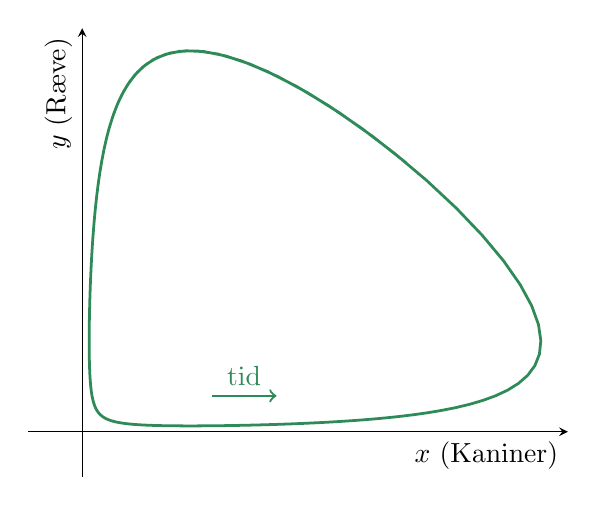
\begin{tikzpicture}
	\begin{axis}[
		axis lines = center, 
		xmin = -0.5, xmax = 4.5,
		ymin = -0.5, ymax = 4.5,
		xlabel = $x$ (Kaniner),
		ylabel = $y$ (Ræve), 
		xlabel style={
        at={(axis cs:4.5,0)},
        anchor=north east},
		ylabel style={
        at={(axis cs:0,4.5)},
        anchor=south east,
		rotate = 90},
		ticks = none
	]
	
 	\addplot[color = SeaGreen,line width=1.0pt,line join=round] coordinates {
    (3,3)
    (2.694636902,3.29041598)
    (2.386961576,3.553873127)
    (2.088594164,3.780539056)
    (1.808851994,3.963825379)
    (1.554079221,4.100749094)
    (1.327617817,4.191634605)
    (1.130250936,4.239381563)
    (0.960876992,4.248572626)
    (0.817204904,4.224638891)
    (0.696341868,4.173202805)
    (0.595224243,4.099631111)
    (0.51089563,4.008775726)
    (0.440661933,3.904857489)
    (0.382159269,3.791445738)
    (0.333366371,3.671494734)
    (0.292585413,3.547408781)
    (0.258407488,3.421117723)
    (0.229672854,3.294151983)
    (0.205431706,3.167711483)
    (0.18490837,3.042726003)
    (0.167470104,2.919906479)
    (0.152600694,2.799787713)
    (0.139878536,2.682763453)
    (0.128958676,2.569114932)
    (0.11955822,2.459033941)
    (0.111444545,2.352641409)
    (0.104425796,2.250002328)
    (0.098343254,2.151137709)
    (0.093065194,2.05603418)
    (0.088481944,1.964651663)
    (0.084501905,1.876929527)
    (0.081048343,1.792791526)
    (0.078056791,1.712149743)
    (0.075472939,1.634907759)
    (0.073250928,1.560963191)
    (0.071351949,1.490209717)
    (0.069743105,1.422538695)
    (0.068396472,1.357840457)
    (0.067288329,1.296005328)
    (0.066398523,1.23692444)
    (0.065709943,1.180490362)
    (0.065208082,1.126597596)
    (0.064880678,1.075142949)
    (0.064717405,1.026025824)
    (0.064709624,0.979148424)
    (0.064850173,0.9344159)
    (0.065133183,0.89173645)
    (0.065553932,0.851021372)
    (0.066108722,0.812185089)
    (0.066794768,0.775145149)
    (0.067610112,0.7398222)
    (0.06855355,0.70613995)
    (0.069624565,0.674025112)
    (0.070823278,0.643407345)
    (0.072150404,0.614219181)
    (0.073607216,0.586395944)
    (0.075195514,0.559875674)
    (0.076917604,0.534599043)
    (0.078776276,0.510509265)
    (0.080774795,0.48755201)
    (0.082916882,0.465675322)
    (0.085206716,0.444829527)
    (0.087648924,0.424967149)
    (0.090248584,0.406042827)
    (0.093011221,0.388013232)
    (0.095942817,0.370836987)
    (0.099049813,0.354474584)
    (0.102339116,0.338888314)
    (0.105818114,0.324042189)
    (0.109494683,0.30990187)
    (0.1133772,0.2964346)
    (0.117474564,0.283609134)
    (0.121796206,0.271395676)
    (0.126352111,0.259765818)
    (0.131152838,0.248692478)
    (0.136209542,0.238149845)
    (0.141533994,0.22811332)
    (0.14713861,0.218559468)
    (0.153036477,0.209465966)
    (0.159241379,0.20081155)
    (0.165767826,0.192575978)
    (0.172631092,0.184739976)
    (0.17984724,0.177285204)
    (0.187433163,0.170194209)
    (0.195406619,0.163450392)
    (0.203786271,0.15703797)
    (0.212591726,0.150941939)
    (0.221843577,0.145148047)
    (0.231563453,0.139642755)
    (0.24177406,0.134413216)
    (0.252499234,0.129447241)
    (0.263763991,0.124733277)
    (0.27559458,0.12026038)
    (0.288018538,0.116018194)
    (0.301064754,0.111996929)
    (0.31476352,0.108187342)
    (0.329146603,0.104580719)
    (0.344247305,0.101168859)
    (0.360100533,0.097944058)
    (0.376742868,0.094899097)
    (0.394212639,0.092027234)
    (0.412549997,0.089322187)
    (0.431796993,0.086778137)
    (0.451997657,0.084389713)
    (0.473198079,0.082151996)
    (0.495446492,0.080060515)
    (0.518793358,0.07811125)
    (0.543291454,0.076300638)
    (0.568995956,0.07462558)
    (0.595964529,0.073083452)
    (0.624257412,0.071672123)
    (0.653937503,0.070389973)
    (0.685070444,0.069235922)
    (0.717724699,0.068209457)
    (0.75197163,0.067310675)
    (0.787885567,0.066540326)
    (0.825543866,0.06589987)
    (0.865026957,0.065391545)
    (0.906418384,0.065018443)
    (0.949804816,0.064784609)
    (0.99527604,0.064695147)
    (1.042924934,0.064756362)
    (1.092847388,0.06497591)
    (1.145142198,0.065362992)
    (1.199910895,0.06592858)
    (1.257257512,0.066685683)
    (1.317288273,0.067649673)
    (1.380111172,0.068838669)
    (1.445835441,0.070274007)
    (1.514570852,0.071980797)
    (1.586426846,0.073988604)
    (1.661511414,0.076332276)
    (1.739929706,0.079052943)
    (1.821782277,0.082199242)
    (1.907162892,0.085828818)
    (1.996155787,0.090010163)
    (2.088832249,0.094824879)
    (2.185246345,0.100370477)
    (2.285429595,0.106763838)
    (2.389384321,0.1141455)
    (2.497075347,0.122684989)
    (2.608419639,0.132587447)
    (2.723273379,0.144101873)
    (2.841415852,0.15753137)
    (2.9625294,0.173245848)
    (3.086174553,0.191697734)
    (3.211759334,0.213441238)
    (3.338501629,0.239155791)
    (3.465383578,0.269674105)
    (3.591097126,0.306015044)
    (3.713980535,0.349420823)
    (3.831946927,0.401396873)
    (3.942408217,0.463750606)
    (4.042201684,0.538621999)
    (4.127532327,0.628493954)
    (4.193952553,0.736163636)
    (4.236411117,0.864648062)
    (4.249413733,1.016990126)
    (4.227343335,1.195929727)
    (4.164980045,1.403416442)
    (4.058227813,1.639974965)
    (3.904987935,1.903998141)
    (3.706024522,2.191126391)
    (3.465576415,2.493942953)
    (3.191443801,2.802215333)
    (2.894373512,3.103796698)
    (2.586785788,3.386078072)
    (2.281137448,3.637650059)
    (1.988362262,3.849726613)
    (1.716780443,4.016974751)
    (1.471661665,4.137628766)
    (1.255386685,4.213009652)
    (1.067998848,4.246707125)
    (0.90790566,4.243687556)
    (0.772546677,4.209512818)
    (0.658928703,4.149756418)
    (0.564001,4.06962636)
    (0.484886375,3.973761475)
    (0.419001807,3.866153707)
    (0.364103727,3.750151429)
    (0.3182871,3.628508545)
    (0.279959384,3.503454888)
    (0.247803293,3.376772471)
    (0.220736748,3.249868839)
    (0.197874621,3.123843146)
    (0.178494469,2.999543347)
    (0.162007019,2.877614407)
    (0.147931385,2.758538222)
    (0.135874597,2.642666292)
    (0.125514884,2.53024623)
    (0.116588126,2.421443166)
    (0.108876918,2.316356954)
    (0.102201767,2.215035996)
    (0.096414013,2.117488308)
    (0.091390143,2.0236904)
    (0.087027208,1.933594385)
    (0.083239133,1.847133669)
    (0.079953738,1.764227524)
    (0.077110319,1.684784739)
    };
	\draw[color = SeaGreen, thick, ->] (axis cs: 1.2,0.4) -- (axis cs: 1.8, 0.4) node[pos = 0.5, anchor = south] {tid};
	\end{axis}		
	\end{tikzpicture}
	\caption{Fasediagram for rovdyr-byttedyr-modellen med kaniner og ræve.}
	\label{fig:fasediagram}
\end{figure}
Vi kan på figuren se, at der er en cyklisk sammenhæng mellem antallet af kaniner og antallet af ræve. Antallet af kaniner vokser, hvilket får antallet af ræve til at vokse, hvilket får antallet af kaniner til at falde, hvilket får antallet af ræve til at falde som til slut så får antallet af kaniner til at stige igen. 
På Figur \ref{fig:tidsplot} kan vi se, hvordan antallet af ræve og kaniner afhænger af tiden.
\begin{figure}[H]
	\centering
	\resizebox{0.49\textwidth}{!}{
	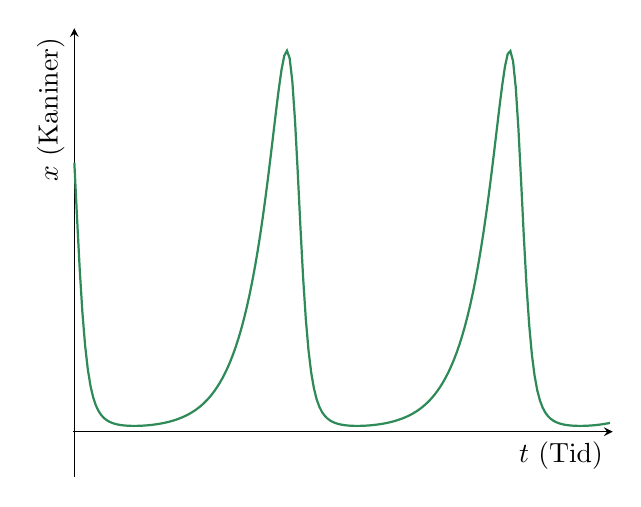
\begin{tikzpicture}
	\begin{axis}[
		axis lines = center, 
		xmin = -0.5, xmax = 200,
		ymin = -0.5, ymax = 4.5,
		xlabel = $t$ (Tid),
		ylabel = $x$ (Kaniner), 
		xlabel style={
        at={(axis cs:200,0)},
        anchor=north east},
		ylabel style={
        at={(axis cs:0,4.5)},
        anchor=south east,
		rotate = 90},
		ticks = none
	]
	\addplot[SeaGreen, thick] coordinates {
    (0,3)
    (1,2.386961575)
    (2,1.808851994)
    (3,1.327617819)
    (4,0.960876996)
    (5,0.696341873)
    (6,0.510895635)
    (7,0.382159273)
    (8,0.292585417)
    (9,0.229672857)
    (10,0.184908372)
    (11,0.152600696)
    (12,0.128958677)
    (13,0.111444546)
    (14,0.098343255)
    (15,0.088481945)
    (16,0.081048344)
    (17,0.07547294)
    (18,0.07135195)
    (19,0.068396473)
    (20,0.066398524)
    (21,0.065208083)
    (22,0.064717405)
    (23,0.064850174)
    (24,0.065553933)
    (25,0.066794768)
    (26,0.06855355)
    (27,0.070823278)
    (28,0.073607217)
    (29,0.076917605)
    (30,0.080774795)
    (31,0.085206717)
    (32,0.090248585)
    (33,0.095942818)
    (34,0.102339117)
    (35,0.109494684)
    (36,0.117474565)
    (37,0.126352112)
    (38,0.136209543)
    (39,0.147138612)
    (40,0.15924138)
    (41,0.172631093)
    (42,0.187433164)
    (43,0.203786273)
    (44,0.221843579)
    (45,0.241774062)
    (46,0.263763993)
    (47,0.288018541)
    (48,0.314763523)
    (49,0.344247308)
    (50,0.376742871)
    (51,0.41255)
    (52,0.45199766)
    (53,0.495446496)
    (54,0.543291458)
    (55,0.595964534)
    (56,0.653937508)
    (57,0.717724704)
    (58,0.787885573)
    (59,0.865026964)
    (60,0.949804822)
    (61,1.042924941)
    (62,1.145142206)
    (63,1.257257521)
    (64,1.380111182)
    (65,1.514570863)
    (66,1.661511425)
    (67,1.821782289)
    (68,1.9961558)
    (69,2.185246359)
    (70,2.389384336)
    (71,2.608419654)
    (72,2.841415868)
    (73,3.086174569)
    (74,3.338501645)
    (75,3.59109714)
    (76,3.83194694)
    (77,4.042201693)
    (78,4.193952558)
    (79,4.249413732)
    (80,4.164980035)
    (81,3.904987915)
    (82,3.465576384)
    (83,2.894373474)
    (84,2.281137411)
    (85,1.716780411)
    (86,1.255386663)
    (87,0.907905647)
    (88,0.658928696)
    (89,0.484886371)
    (90,0.364103725)
    (91,0.279959383)
    (92,0.220736747)
    (93,0.178494469)
    (94,0.147931386)
    (95,0.125514884)
    (96,0.108876919)
    (97,0.096414013)
    (98,0.087027208)
    (99,0.079953738)
    (100,0.074657698)
    (101,0.070758466)
    (102,0.067983349)
    (103,0.066135898)
    (104,0.065074446)
    (105,0.064697411)
    (106,0.064933114)
    (107,0.06573267)
    (108,0.067064983)
    (109,0.068913207)
    (110,0.071272249)
    (111,0.074147022)
    (112,0.077551234)
    (113,0.081506592)
    (114,0.086042312)
    (115,0.091194867)
    (116,0.09700794)
    (117,0.103532521)
    (118,0.110827154)
    (119,0.118958301)
    (120,0.128000819)
    (121,0.138038539)
    (122,0.149164958)
    (123,0.161484024)
    (124,0.175111035)
    (125,0.190173638)
    (126,0.206812951)
    (127,0.225184796)
    (128,0.245461066)
    (129,0.26783121)
    (130,0.292503874)
    (131,0.319708674)
    (132,0.349698124)
    (133,0.382749718)
    (134,0.419168166)
    (135,0.459287784)
    (136,0.503475014)
    (137,0.552131079)
    (138,0.605694717)
    (139,0.664644948)
    (140,0.729503799)
    (141,0.800838848)
    (142,0.879265418)
    (143,0.965448142)
    (144,1.060101494)
    (145,1.163988703)
    (146,1.277918155)
    (147,1.40273598)
    (148,1.539312852)
    (149,1.688521974)
    (150,1.851203694)
    (151,2.028109627)
    (152,2.21981525)
    (153,2.426583659)
    (154,2.648153347)
    (155,2.883407689)
    (156,3.129861534)
    (157,3.38287093)
    (158,3.634443904)
    (159,3.871537377)
    (160,4.073868542)
    (161,4.211782201)
    (162,4.245971274)
    (163,4.132890465)
    (164,3.840538753)
    (165,3.373141699)
    (166,2.787463183)
    (167,2.176908405)
    (168,1.627964592)
    (169,1.186695407)
    (170,0.8579565)
    (171,0.623794778)
    (172,0.460488604)
    (173,0.347153664)
    (174,0.268084429)
    (175,0.212312293)
    (176,0.172432624)
    (177,0.143507821)
    (178,0.122245553)
    (179,0.106435457)
    (180,0.094577812)
    (181,0.085642504)
    (182,0.078912986)
    (183,0.073884811)
    (184,0.070199093)
    (185,0.067598395)
    (186,0.065897155)
    (187,0.064961618)
    (188,0.064696055)
    (189,0.065033214)
    (190,0.065927627)
    (191,0.06735091)
    (192,0.069288424)
    (193,0.071736934)
    (194,0.074702962)
    (195,0.078201661)
    (196,0.082256078)
    (197,0.086896708)
    (198,0.092161284)
    (199,0.098094752)
};

	\end{axis}		
	\end{tikzpicture}
	}
	\resizebox{0.49\textwidth}{!}{
	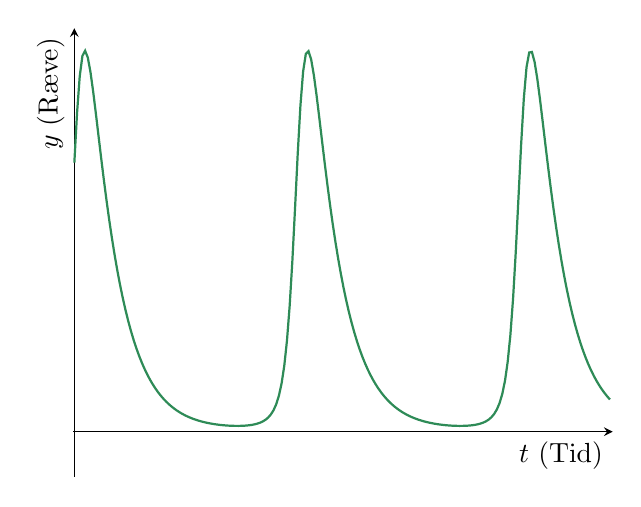
\begin{tikzpicture}
	\begin{axis}[
		axis lines = center, 
		xmin = -0.5, xmax = 200,
		ymin = -0.5, ymax = 4.5,
		xlabel = $t$ (Tid),
		ylabel = $y$ (Ræve), 
		xlabel style={
        at={(axis cs:200,0)},
        anchor=north east},
		ylabel style={
        at={(axis cs:0,4.5)},
        anchor=south east,
		rotate = 90},
		ticks = none
	]
	\addplot[SeaGreen, thick] coordinates {
(0,3)
(1,3.553873129)
(2,3.963825381)
(3,4.191634606)
(4,4.248572626)
(5,4.173202803)
(6,4.008775724)
(7,3.791445737)
(8,3.547408781)
(9,3.294151984)
(10,3.042726004)
(11,2.799787714)
(12,2.569114933)
(13,2.352641411)
(14,2.151137711)
(15,1.964651664)
(16,1.792791528)
(17,1.634907761)
(18,1.490209719)
(19,1.357840458)
(20,1.236924442)
(21,1.126597597)
(22,1.026025825)
(23,0.934415902)
(24,0.851021373)
(25,0.775145151)
(26,0.706139951)
(27,0.643407347)
(28,0.586395945)
(29,0.534599044)
(30,0.487552011)
(31,0.444829528)
(32,0.406042828)
(33,0.370836987)
(34,0.338888315)
(35,0.309901871)
(36,0.283609135)
(37,0.259765819)
(38,0.238149845)
(39,0.218559469)
(40,0.200811551)
(41,0.184739977)
(42,0.170194209)
(43,0.15703797)
(44,0.145148047)
(45,0.134413217)
(46,0.124733277)
(47,0.116018194)
(48,0.108187342)
(49,0.101168859)
(50,0.094899098)
(51,0.089322188)
(52,0.084389713)
(53,0.080060515)
(54,0.076300639)
(55,0.073083452)
(56,0.070389974)
(57,0.068209458)
(58,0.066540326)
(59,0.065391545)
(60,0.064784609)
(61,0.064756363)
(62,0.065362993)
(63,0.066685684)
(64,0.06883867)
(65,0.071980798)
(66,0.076332278)
(67,0.082199243)
(68,0.090010164)
(69,0.100370479)
(70,0.114145502)
(71,0.13258745)
(72,0.157531373)
(73,0.191697739)
(74,0.239155797)
(75,0.306015052)
(76,0.401396884)
(77,0.538622014)
(78,0.736163656)
(79,1.01699015)
(80,1.403416472)
(81,1.903998176)
(82,2.493942991)
(83,3.103796734)
(84,3.637650088)
(85,4.01697477)
(86,4.213009659)
(87,4.243687552)
(88,4.149756407)
(89,3.973761461)
(90,3.750151413)
(91,3.503454871)
(92,3.249868823)
(93,2.999543333)
(94,2.758538209)
(95,2.530246218)
(96,2.316356943)
(97,2.117488298)
(98,1.933594376)
(99,1.764227516)
(100,1.608706544)
(101,1.466224763)
(102,1.335919138)
(103,1.216914359)
(104,1.10835051)
(105,1.009400016)
(106,0.919277508)
(107,0.837245041)
(108,0.762614241)
(109,0.694746457)
(110,0.633051627)
(111,0.576986345)
(112,0.52605145)
(113,0.479789377)
(114,0.437781391)
(115,0.399644829)
(116,0.365030408)
(117,0.333619634)
(118,0.305122344)
(119,0.279274405)
(120,0.25583555)
(121,0.234587383)
(122,0.21533153)
(123,0.197887935)
(124,0.182093307)
(125,0.167799688)
(126,0.154873166)
(127,0.143192697)
(128,0.13264905)
(129,0.123143857)
(130,0.114588779)
(131,0.106904766)
(132,0.100021425)
(133,0.093876498)
(134,0.088415435)
(135,0.083591098)
(136,0.079363587)
(137,0.075700212)
(138,0.072575646)
(139,0.069972297)
(140,0.067880941)
(141,0.06630173)
(142,0.065245652)
(143,0.064736653)
(144,0.064814629)
(145,0.065539669)
(146,0.066998068)
(147,0.069310897)
(148,0.072646335)
(149,0.077237557)
(150,0.083409025)
(151,0.091615538)
(152,0.102500953)
(153,0.116987443)
(154,0.136412466)
(155,0.162740175)
(156,0.198887698)
(157,0.249223326)
(158,0.320304523)
(159,0.421897985)
(160,0.568176164)
(161,0.778525257)
(162,1.076356113)
(163,1.482782135)
(164,2.001992024)
(165,2.601608006)
(166,3.20522712)
(167,3.71657537)
(168,4.064409921)
(169,4.229285575)
(170,4.235000482)
(171,4.12382886)
(172,3.937319906)
(173,3.708173399)
(174,3.459305523)
(175,3.205695036)
(176,2.956651445)
(177,2.717680667)
(178,2.491819494)
(179,2.280532338)
(180,2.084296719)
(181,1.902980859)
(182,1.736086234)
(183,1.582903279)
(184,1.442611321)
(185,1.314342561)
(186,1.197222742)
(187,1.090396618)
(188,0.993043428)
(189,0.904385815)
(190,0.823694407)
(191,0.750289548)
(192,0.683541182)
(193,0.622867554)
(194,0.567733168)
(195,0.517646327)
(196,0.472156445)
(197,0.430851288)
(198,0.393354214)
(199,0.359321502)
};
	\end{axis}		
	\end{tikzpicture}
	}
	\caption{Sammenhæng mellem den forløbne tid og koncentrationen af både kaniner og ræve.}
	\label{fig:tidsplot}
\end{figure}
Vi kan på Figur \ref{fig:tidsplot} også se, hvordan antallet af kaniner og ræve stiger og falder cyklisk som funktion af tiden. 

Det er som udgangspunkt ikke ræve og kaniner, der har vores interesse, men derimod økonomiske modeller. Det viser sig dog, at \textit{Goodwin-modellen} beskriver sammenhængen mellem beskæftigelse og lønniveau på en måde, der opfører sig nøjagtigt som rævene og kaninerne på vores isolerede ø.

\section*{Goodwin-modellen}
\stepcounter{section}





\end{document}